\documentclass{article}
\usepackage{array} % for custom column widths
\usepackage{booktabs} % for better-looking tables
\usepackage{graphicx} % Required for inserting images
\usepackage{geometry}
\usepackage{graphicx}
\usepackage{subcaption}
\usepackage{float} % Required for 'H' placement specifier
\usepackage{hyperref} % Include the hyperref package

\title{QF634 Report : Beyond Conventional Charts: Signal Processing Indicators as Catalysts for Predicting Peaks/Troughs in Forex Trading}
\author{Andre LIM, LIU YiSi, Dylan LOO, WANG WenJie}
\date{December 2023}

\begin{document}

\maketitle

\section{Introduction}

\subsection{Thesis Statement}
The objective of our project is to answer a key question using ML methods: \textit{Can non-traditional technical indicators (such as Fourier Transform, Kalman Filter, Hurst Exponent (also known as Signal Processing Indicators)) be used in conjunction with traditional technical indicators to boost the performance of ML models to predict buy / sell signal in forex markets?} Through this project we aim to answer this question, while experimenting with additional variables and features that were deemed to have potential to boost the performance of the final model.
\newline
\newline
\noindent In the final implementation, we used a trading time frame of 2013 to 2023. During this period, the value of JPY in USD terms dropped by about 41\%, which made for an interesting challenge. Source code to our project can be found in our github repository: \href{https://github.com/andreignatius/quantresearch}{https://github.com/andreignatius/quantresearch}.

\begin{figure}[h]
  \centering
  \includegraphics[scale=0.6]{usd_jpy_2000_2024.PNG}
  \caption{USD/JPY Exchange Rate From the mid 90s to the mid 20s}
\end{figure}

\noindent In order to generate our optimal peaks and troughs, we used the  \texttt{scipy.signal.find\_peaks} package in Python. At this juncture, it would be pertinent to highlight that in the actual implementation, we assess the performance of the model \textit{not by its ability to perfectly predict} optimal peaks and troughs, but its ability to \textit{consistently make good predictions} that are close enough to local market peaks and troughs such that each trade results in positive PnL,  each holding period does not incur significant downside risk and that PnL is maximised.
\newline

\begin{figure}[h]
  \centering
  \includegraphics[scale=0.28]{peak_detection.png}
  \caption{Peak/Trough Labeling using scipy.signal.find\_peaks for USD/JPY Spot Rate from November 2022 to November 2023}
\end{figure}

\noindent Before proceeding, it also is worth disclaiming that the prices we used to determine optimal buy/hold/sell days were the 'Closing' price of the trading pair. Since the forex market is open 24 hours a day, precision of the definition of 'Close' price is important: The closing price in forex typically signifies the final price at the end of a trading session. For instance, if we were in the GMT time zone, the New York market close (around 5:00 PM EST or 10:00 PM GMT) is often considered the end of the trading day. The price at this point is recorded as the closing price for that particular day.

\subsection{Theoretical Background}
Hurst postulated that financial time series data could be modelled as a combination of discrete harmonic frequencies. This concept is part of the broader field of cyclical analysis, where financial market time series are considered to have a cyclical nature that can be decomposed into a series of sinusoidal components or waves, each with their own frequency, amplitude, and phase. These components correspond to different cycles that are superimposed upon each other, creating the observed market movements.
\newline
\newline
To help visualise the concept, let us take example of a musical chord, the A major chord with its triad A5, C\(\sharp\)5, E5.
\newline

\begin{figure}[h]
  \centering
  \begin{subfigure}{0.4\textwidth}
    \centering
    \includegraphics[scale=0.6]{a_maj_chord.png}
    \caption{A major chord}
  \end{subfigure}
  \hspace{0.1\textwidth} % Adjust the horizontal space between images as needed
  \begin{subfigure}{0.4\textwidth}
    \centering
    \includegraphics[scale=0.6]{a_note.png}
    \caption{Fundamental A note}
  \end{subfigure}
  \caption{A major chord and fundamental A note}
  \label{fig:a_major_chord_note}
\end{figure}

\noindent The A major chord wave is a combination of 3 other individual sinusoidal waves, note A at 880Hz, C\(\sharp\) at 1100Hz, E at 1320Hz (values modified under different tuning system to reflect whole numbers). At the individual note level, the wave pattern appears clearly sinusoidal but when combined it looks noisier and more convoluted.

\noindent Let us examine with another visual example, how different notes add up to form a chord. This time with G major chord, with its continuent G3, B3, D3 notes (again the values are modified under different tuning system to reflect whole numbers).

\begin{figure}[h]
    \centering
    \includegraphics[scale=0.7]{g_maj_chord.png}
    \caption{Visualization of fundamental notes combining together to form the G major musical chord}
    \label{fig:gmajchord}
\end{figure}


\noindent There are several observations and postulations in Hurst Cycle Theory
\begin{enumerate}
\item Cyclical Nature: Hurst observed that many systems exhibit cycles in a nested fashion, where smaller cycles exist within larger ones. This concept was originally applied to the analysis of river Nile floods but has since been extended to financial markets.
\item Predictability: The cycles are not perfectly periodic but have a degree of predictability. By identifying the cycle lengths, one can forecast the future movement of a time series to some extent.
\item Mean Reversion and Trend: The Hurst exponent (H) is a key outcome of his work, which measures the tendency of a time series to revert to its mean (H \(<\) 0.5), to trend (H \(>\) 0.5), or to follow a random walk (H = 0.5).
\item Market Analysis: In financial markets, Hurst Cycle Theory is used to identify potential market cycles for both short-term and long-term trading strategies. Traders and analysts look for patterns that repeat over time and use them to forecast market movements.
\item Fractal Nature: The theory also suggests that financial markets are fractal in nature. This means that market patterns can be self-similar at different scales, which is the basis for fractal market analysis.
\item Sentiment and Fundamentals: Hurst cycles can be influenced by market sentiment and fundamentals. For example, economic indicators, geopolitical events, and trader psychology can all influence the length and amplitude of cycles.
\end{enumerate}

\subsection{Motivations \& Intuition}
\subsubsection{Why do forex movements matter (to an average person)?}
In this globalized economy, many talented individuals are willing to leave their hometown to seek work opportunities abroad. However, a pressing concern remains for these migrant talent that their hard-earned income could be vulnerable to unfavourable forex movements, especially when they try to remit allowance back home or if they intend to return to their country of origin after a certain number of years.
\newline
\newline
\noindent To better illustrate this concern, let us take the example of a fictional character, Chad Nakamura. Chad Nakamura is an American citizen who found a job in Tokyo in 2013 and left the United States to start his career. As an Asian American with good Japanese language skills, it made sense to make the move.
\newline
\newline
\noindent Chad starts out in Tokyo with annual salary of 6.500.000 JPY which equates to 75.000 USD at the time of exchange rate on 1 Jan 2013 to work for Yoshi \& Co. Over his time in the company, he got the following progression: he got annual increments of 2\% per annum for good performance and 10\% increment for promotions in 2016, 2018, 2021 and 2023. By 2023, his salary in JPY is now 65\% higher than when he first start at Yoshi \& Co. back in 2013.
\newline
\newline
\noindent He will learn however that the celebration is short-lived, as the fruits of his hard labour were been eroded by forex movements against his favour. Because in the same period, USD/JPY spot rate moved from 86.64 to 130.85.
\newpage
\begin{figure}[h]
  \centering
  \includegraphics[scale=0.45]{chad_jpy_salary.png}
  \caption{Chad's salary progression in JPY from 2013 to 2023}
  \label{fig:chad_salary}
\end{figure}

\begin{figure}[h]
  \centering
  \includegraphics[scale=0.45]{usd_salary_0.png}
  \caption{Chad's salary progression in USD from 2013 to 2023}
  \label{fig:chad_salary}
\end{figure}

\noindent In 2013 his salary of 6.500.000 JPY was worth 75.000 USD. However, his 2023 salary of 10.717.294 JPY is worth 73.984 USD. Throughout the sweat, tears and blood, Chad's salary when converted to his domestic currency in USD actually suffered -1.35\% loss. This loss is extra devastating when one considers that it has not yet been adjusted for inflation.
\newline
\newline
Chad's story, along with many others like him, motivated us to create an automated trading strategy to hedge against forex movements and generate alpha.
\newpage
\subsubsection{Intuition from Theory (what can we do about it?)}
Given what we have read from Hurst Cycle Theory and if we hold the postulate that financial time series data is as a combination of discrete harmonic frequencies, we can then align our research to explore various techniques in signal processing, such as Fourier transform, which breaks down time series into sinusoidal components. In the next chapter, we will explore the available signal processing techniques in greater depth.

\section{Feature Generation}

\subsection{Signal Processing Indicators}

\subsubsection{Fourier Transform}

\textit{What is it about?}
Fourier transform is a mathematical technique that decomposes a complex signal into its constituent frequencies. The applied areas include signal processing, image analysis and sound decomposition etc. In financial industry, Fourier transform is utilised to convert the time series price data to dominant periodic trends. 
\newline
\newline
\(F(\omega) = \int_{-\infty}^{\infty} f(t) e^{-i \omega t} \, dt\), where F(\(\omega\)) is the Fourier transformation of time series data f(t). It tells us how much each frequency is presented in the time series data.
\newline
\newline
\textit{Intuition as feature:}
There are two domains in Fourier transformation: time-domain and frequency domain. In our case, Fourier transform takes time domain signal (Forex price) and converts it to frequency domain signal (the cyclical signal). The frequency domain signal shows the frequency components that dominate the price data.
\newline

\begin{figure}[h]
  \centering
  \includegraphics[scale=0.2]{fourier_frequencies.png}
  \caption{Dominant frequencies in USD/JPY Close Prices from Nov 2022 to Nov 2023}
\end{figure}

\begin{figure}[h]
  \centering
  \includegraphics[scale=0.2]{fourier_cycles.png}
  \caption{Dominant period cycles in USD/JPY Close Prices from Nov 2022 to Nov 2023}
\end{figure}
\newpage
\subsubsection{Kalman Filter}

\textit{What is it about?}
Kalman Filter is a useful time series analysis algorithm in financial industry. Compared to Simple Moving Average, Kalman Filter puts more weight on more recent data on the calculation and takes statistical noises into consideration.  
\newline
\newline
Kalman Filter works with two phases: the prediction phase and update phase. The prediction phase estimates the state at current timestamp. In the update phase, the innovation (difference between current prediction and current observation) is multiplied by Kalman gain (the weightage to most recent data) and combined with previous state estimation. This refined estimate is termed the posteriori state estimate.
\newline
\newline
The algorithm is a recursive process, thus can operate in real time. And it assumes the errors have a normal distribution. 
\newline
\newline
\textit{Intuition as feature:}
Using Kalman Filter algorithm, we can derive the optimal state estimate of Forex spot rate combining prediction phase and update phase in a recursive process. This optimal state estimate gives us a smoothed and unbiased Forex spot rate which sifted out the unnecessary noise. The volatility (deviation from mean) can also be derived from Kalman Filter algorithm  


\subsubsection{Hurst Exponent}

\textit{What is it about?}
Hurst Exponent is a mathematical measure of the long-term memory of a time series data that tells us the persistence of trend. First developed by Harold Edwin Hurst to solve the optimal dam size issue on Nile river, Hurst Exponent indicates us whether a time series is purely random, trending or mean reversion.
\newline
\newline
The equation for Hurst Exponential is: \(E\left[\frac{R(n)}{S(n)}\right] = Cn^H\)
\newline
where R(n) is the range of first n cumulative deviations from the mean, S(n) is the series of first n standard deviations, n is the span of the observation and C is a constant.
\newpage
The most generic interpretation of Hurst Exponential is:
\begin{enumerate}
\item When H \(<\) 0.5, the time series is mean reverting, which indicates an anti-persistent behaviour
\item When H = 0.5, the time series exhibits Brownian motion with pure random walk
\item When H \(>\) 0.5, the time series is trending with a certain degree of predictability, which indicates a persistent behaviour
\end{enumerate}

\begin{figure}[h]
  \centering
  \begin{subfigure}{0.3\textwidth}
    \centering
    \includegraphics[width=\textwidth]{hurst_lesser_0_5.png}
    \caption{Hurst Exponent $<$ 0.5}
  \end{subfigure}
  \hspace{0.05\textwidth} % Adjust the horizontal space between images as needed
  \begin{subfigure}{0.3\textwidth}
    \centering
    \includegraphics[width=\textwidth]{hurst_greater_0_5.png}
    \caption{Hurst Exponent $>$ 0.5}
  \end{subfigure}
  \hspace{0.05\textwidth} % Adjust the horizontal space between images as needed
  \begin{subfigure}{0.3\textwidth}
    \centering
    \includegraphics[width=\textwidth]{hurst_0_5.png}
    \caption{Hurst Exponent = 0.5}
  \end{subfigure}
  \caption{Simulation of fractional Brownian motion for different values of the Hurst exponent}
\end{figure}

\noindent
\textit{Intuition as feature:}
Hurst Exponent tells us the domain of the current time series of Forex spot rate. We can use it to assess the essence of price movements. It gives us the information of whether the time series is currently mean-reverting or trending, and allows us to execute different strategies accordingly. 

\subsection{First and Second Order Derivatives of Indicators}
\textit{What is it about and why does it matter?} It should be noted that during this experiment, that identifying the best spot price to trade is not as important as \textbf{identifying the trend reversal turning point} of the spot price. The spot price data on its own has little predictive value without any reference to the date it belongs to but the date itself also has little value in predictive power as a date, once passed, will never repeat itself again.
\newline
\newline
\textit{Intuition as feature:} Thus, the intuition came about that we were more interested in rate of change (first order derivative) or rate of rate of change (second order derivative) of the spot price in trying to time our trades in the spot market. For certain technical indicators like \textbf{Kalman Filter Estimate} and \textbf{Short / Long Moving Averages}, it made sense to compute the \textbf{first and second order derivative} values of those features and set those values as a new indicator.

\subsection{Exogenous Economic Indicators}
Spot forex exchange rate between JPY and USD is affected by several econometrics, such as the country's base rate, inflation, currency account balance, capital inflow and monetary policies in Japan and US. The correlation between exogenous variables and the USD/JPY forex rate is analysed in our model.
\subsubsection{Uncovered Interest Rate Parity}
Uncovered interest rate parity states that the expected change in spot exchange rate is equal to the interest rate differential between two countries. This theory does not involve the use of forward contracts and assumes the investor is risk-neutral.
\newline
The equation is: 
\(E[S_{t+1}] = S_t \times \frac{1+I_{Japan}}{1+I_{USA}} \)
\newline
\newline
The expected spot USD/JPY forex exchange rate is determined by multiplying the current USD/JPY forex exchange rate with the ratio of the baseline interest rate in Japan to the baseline interest rate in the US.
\subsubsection{Relative Purchasing Power Parity}
The relative purchasing power parity (PPP) is based on the theory of law of one price, which states that without the transportation costs and other frictions, identical goods should have the same price in all countries. And relative PPP extends this concept and states that changes in exchange rates should exactly offset the price effects of any inflation differential between 2 countries.
\newline
\newline
The equation is: \(\frac{E[S_{t+1}]}{S_t} = \frac{1+Inflation in Japan}{1+Inflation in USA} \)
\newline
\newline
The expected change of spot USD/JPY forex exchange rate is equal to the ratio of inflation rate in Japan to inflation rate in US.
\newline
\newline
The relative PPP assumes long-term equilibrium, while in short run, other factors like speculative activities may affect the forex rate.


\subsubsection{Current Account Balance}

The current account provides a comprehensive overview of a country's trade, encompassing the exchange of goods, services, investment income, and unilateral transfers. It serves as a concise indicator of whether a nation is exporting more goods and services than it imports, thus signaling either a current account surplus or deficit.
\newline
\newline
Current account deficits lead to a depreciation of domestic currency because:
\begin{itemize}
\item Flow supply/demand mechanism: current account deficits in a country increase the supply of that currency in the currency markets, it puts downward pressure on the exchange value of the currency. 
\item Portfolio balance mechanism: countries with current account surpluses usually have capital account deficits, which typically take the form of investments in countries with current account deficits. When investor countries decide to rebalance their investment portfolios, it can have a significant negative impact on the value of those investee country currency.
\end{itemize}

\subsubsection{Capital Flows}

Capital flows tend to be the dominant factor influencing exchange rates in the short term, as capital flows tend to be larger and more rapidly changing than goods flows. 
\newline
\newline
The country with capital account surplus may be running a current account deficit by borrowing from abroad. There will be an issue for debt sustainability, as when the level of debt gets too high relative to GDP, investors may question the sustainability of this level of debt, leading to a rapid depreciation of the borrower’s currency.  

\subsubsection{Mundell Fleming Model}

The model evaluates the short-term impact of monetary and fiscal policies on exchange rates.
\newline
\newline
For our case, USD/JPY forex rate, both Japan and United States have high capital mobility (without capital mobility restriction). Therefore, expansionary monetary policy will decrease the interest rate and reduce the inflows of capital investment in physical and financial assets. The decrease in capital inflows reduces the demand for the domestic currency, resulting in depreciation of the domestic currency.
\newline

\subsubsection{Proxies for Econometric Exogenous Variables}
\begin{table}[h!]
\centering
\begin{tabular}{|l|l|}
\hline
\textbf{Econometric Exogenous Variable} & \textbf{Proxy} \\
\hline
Base Interest Rate & 1Y Sovereign Bond Yield \\
\hline
Inflation & Consumer Price Index (CPI) \\
\hline
Current Account Balance & Currency Account Balance \\
\hline
Capital Inflow & Foreign Direct Investment (FDI) \\
\hline
Monetary Policy & Money Supply (M2) \\
\hline
\end{tabular}
\caption{Proxies for Econometric Exogenous Variables}
\label{table:proxies}
\end{table}


\subsection{Optimized Indicators}
\subsubsection{Traditional Technical Indicators}
Simple Moving Average (SMA): is a trend indicator that smooths out the price data and identifies trends of property price. The calculation is simply by adding up all the data points over a specified period and dividing the sum by number of periods.
\newline
\newline
Exponential Moving Average (EMA): is also a trend indicator that gives us the smoothed out trend of property price. Different from SMA, it allocates more weight to short-term price change, thus can better reflect the latest market trend.
\newline
\newline
Average Directional Index (ADX): is derived from two rudimental indicators: Plus Directional Indicator (+DI) and Minus Directional Indicator (-DI). As a trend indicator, ADX tells us the strength of prevailing trend by calculating the division of Average True Range of DX by Smoothing Period.
\newline
\newline
Bollinger Bands: is a volatility indicator that consists of three lines: N-period SMA, an upper band with K times the N-period SMA deviation above the N-period SMA and a lower band with K times the N-period SMA deviation below the N-period SMA. It is dynamically adjusted to price volatility, and gives the trader signals of overbought and oversold when the middle band crosses the upper band and lower band.
\newline
\newline
Standard Deviation: is a statistical measurement of the variability and dispersion of property’s price around its mean. It provides insights into the volatility of the property’s price, which is associated with the risk and potential price swing. 
\newline
\newline
Rate of Change (ROC): measures the percentage change in price between the current closing price and the closing price a certain number of periods ago. It helps the trader to identify the speed of price movement, which gives the insight of the strength of a trend.
\newline
\newline
Relative Strength Index (RSI): is a momentum indicator that measures the speed and change of price movements. RSI, which oscillates between 0 and 100, is calculated based on Relative Strength (RS) where RS is the average of x days’ up close divided by the average of x days’ down close. It helps the trader to identify the sell signal when RSI crossover upper band and buy signal when RSI crossover lower band.
\newline
\newline
Moving Average Convergence Divergence (MACD): is a momentum indicator which tells us the relation between two moving averages of a security's price. It helps the trader to identify the potential mean reversion (buy and sell signals) when crossover between MACD line and signal line happens. The MACD line is calculated by the difference between two periods’ EMA and the Signal line is calculated by the EMA of the MACD line.
\newline
\newline
Stochastic Oscillator: is a momentum indicator that calculates the closing price of a property over a specific period (normally 14 periods). The stochastic oscillator helps to signal the potential overbought \& oversold and mean reversion. 
\newline
\newline
Momentum: is a momentum indicator which calculates the difference between today’s closing price and N periods’ ago closing price. It gives the trader the indication of momentum of the properties’ price.

\begin{table}[h!]
\centering
\small % Reduce font size
\setlength{\tabcolsep}{6pt} % Adjust column separation
\begin{tabular}{|p{6cm}|p{6cm}|}
\hline
Simple Moving Average (SMA) & Stochastic Oscillator \\
\hline
Exponential Moving Average (EMA) & Bollinger Bands \\
\hline
Relative Strength Index (RSI) & Standard Deviation \\
\hline
Moving Average Convergence Divergence (MACD) & Average Directional Index (ADX) \\
\hline
Rate of Change (ROC) & Momentum \\
\hline
\end{tabular}
\caption{Traditional Technical Indicators}
\label{table:Indicators}
\end{table}

\subsubsection{Optimization of Technical Indicators}
On top of the traditional technical indicators, we aimed to test if there is opportunity to optimise parameters of certain technical indicators in order to generate stronger signal generating features. The technical indicators optimised include:
\newline
\newline
The optimization is performed by systematically varying the above-mentioned parameters within specific ranges. You've utilized a parameter sweep approach where you've defined ranges for each parameter to explore multiple combinations. The backtesting library's optimization function is used to test different combinations of these parameters.
\newline
\newline
After conducting the optimization process, the best combination of parameters obtained for maximizing the strategy's performance is:
\begin{table}[h!]
\centering
\begin{tabular}{|l|l|}
\hline
SMA n = 3 & slowk period = 1 \\
\hline
EMA n = 3 & BB n = 9 \\
\hline
RSI n = 7 & STDDEV n = 14 \\
\hline
short MA = 5 & ADX n = 14 \\
\hline
long MA = 15 & ROC n = 7 \\
\hline
signal MA = 5 & MOM n = 7 \\
\hline
fastk period = 5 &   \\
\hline
\end{tabular}
\caption{Optimal Technical Indicators}
\label{table:Optimization results}
\end{table}
\newline
These optimized parameter values are expected to enhance the strategy's ability to generate buy/sell signals based on the technical indicators, potentially improving overall performance when applied to trading strategies. The optimization aims to strike a balance between responsiveness to market changes, reducing noise, and minimizing false signals, thereby increasing the strategy's robustness and effectiveness.
\newline
\newline
These optimised technical indicators will eventually flow into our feature importance analysis to determine if they outperform the other features in generating buy and sell signal for the USD/JPY trading pair.


\newpage
\section{Model Selection}

\subsection{Selection Process \& Methodology}
For our forex trading strategy, where the primary objective is to classify potential buy or sell points, we need to concentrate on algorithms that excel in classification. Therefore, we conducted a model selection process specifically geared towards identifying the top three classification algorithms that are most effective and relevant for our trading strategy.
\subsubsection{Determine algorithms}

The following classification Machine Learning algorithms were considered:
\begin{itemize}
\item Logistic Regression: A fundamental classification algorithm, typically used for binary classification problems but could be adapted for multi-class classification.
\item Support Vector Machine (SVM): Versatile and powerful, SVM can be used for both classification and regression, but it's particularly well-known for its performance in classification.
\item K-Nearest Neighbors (KNN): A simple, non-parametric, lazy learning algorithm used for classification. It classifies a data point based on how its neighbors are classified.
\item Decision Tree: Primarily used for classification (but can also do regression). It's a tree-like model of decisions and their possible consequences.
\item Extra Trees (Extremely Randomized Trees): Similar to Random Forest, this ensemble method is used for classification and regression, but it randomizes certain decisions and thresholds, hence 'extremely' randomized.
\item Random Forest: An ensemble of Decision Trees, typically used for classification (and regression). It's particularly known for its high accuracy, robustness, and ease of use.
\item Gradient Boosted Trees (GBT): An ensemble boosting method primarily used for classification and regression. It builds the model in a stage-wise fashion and generalizes them by allowing optimization of an arbitrary differentiable loss function.
\item Adaptive Boosting (AdaBoost): A boosting algorithm that can be used with many other types of algorithms to improve performance. The output of the other learning algorithms ('weak learners') is combined into a weighted sum that represents the final output of the boosted classifier.
\end{itemize}

\subsubsection{Model Comparison}

\begin{figure}[H]
  \centering
  \includegraphics[width=0.7\textwidth]{AUC.png}
  \caption{AUC Values of Machine Learning Models}
\end{figure}

Based on the train and test results of different algorithms to compare the performances. We used AUC (area under curve) of training and testing sets to evaluate the performances of different models.


\subsubsection{Selected Models}

After comparing the performance results of different models, we decided to proceed with Logistic Regression and Gradient Boosted Trees as they performed better than the others. For our third model, we went with Neural Nets.

\newpage
\subsection{Choice of ML Models}
\subsubsection{Logistic Regression}

We eventually settled on using a logistic regression model with an elastic net penalty. The loss function for this setup was a combination of the logistic loss and the elastic net regularization.
\newline
\newline
Elastic net is a regularization technique that combines both L1 (Lasso) and L2 (Ridge) penalties. 
\newline
\newline
Logistic Regression typically excels in binary classification tasks, modeling linear relationships and discerning trading signals based on input features. With that being said, LogReg can handle multi-class classification.
\newline
\newline
By default, Logistic Regression in scikit-learn handles multi-class classification using the one-vs-rest (OvR) scheme or the 'multinomial' scheme when the solver supports it. Since we selected to use the 'saga' solver, which supports 'multinomial', it can handle multi-class classification without explicitly setting the multi\_class parameter. The model will thus automatically choose the appropriate strategy based on the data provided. Since our target variables (y\_train and y\_test) contain three classes (\textbf{Buy Hold} and \textbf{Sell}), the model will perform multi-class classification using the 'multinomial' approach. This uses the softmax function for multi-class classification in a single model.
\newline
\newline
The softmax function is used in various multiclass classification methods, including logistic regression and neural networks, as it allows one to handle multiple classes in a probabilistic context. Each output from the softmax function is interpreted as the probability of the corresponding class given the input features.
\newline
\newline
During training, the softmax function is often paired with a cross-entropy loss (also known as log loss), which provides a measure of how different the predicted probabilities are from the actual class labels. This pairing is effective for training classifiers to predict the correct class probabilities.

\subsubsection{Gradient Boosted Trees}

Gradient Boosted Trees (GBT) is an ensemble machine learning technique that builds models in a stage-wise fashion. It involves the creation of a sequence of trees, where each subsequent tree aims to correct the errors made by the previous trees. The trees are added to the model sequentially until no further improvements can be made. It's a powerful technique used for both regression and classification problems.
\newline
\newline
For multi-class classification, Gradient Boosting can be used in two ways:
\begin{itemize}
\item One-vs-Rest (OvR) Scheme: Here, one decision tree is trained per class and is responsible for separating its class from the rest. This approach can be used for multi-class classification, but it can be computationally expensive as it requires training as many models as there are classes.

\item Multiclass LogitBoost: This is a direct extension of boosting to the multiclass case. Instead of fitting a tree per class, it fits a tree per class per iteration but modifies the loss function to be a multinomial deviance, which is a generalization of the binomial or binary deviance to the multiclass case.
\newline
\end{itemize}
Our GBT model uses the second approach. It inherently supports multi-class classification by optimizing the multinomial deviance loss function, which is a generalization of the logistic loss for multiple classes.



\subsubsection{Neutral Network (LSTM): (added)}

Neural Network was not part of the earlier model selection process, but considering that Neural Network is a more advanced and sophisticated model compared to the other more basic ones, we wanted to see whether a more complex model would perform better.
\newline
\newline
Neural networks are a set of algorithms, modeled loosely after the human brain, designed to recognize patterns. They interpret sensory data through a kind of machine perception, labeling, or clustering raw input.
\newline
\newline
Within the context of multi-class classification, neural networks can effectively discriminate between more than two classes. This is typically done by including a final layer with a softmax activation function, which is what we did. The softmax function converts the output of the last neural network layer (which could be in any range depending on the previous activation functions) into a probability distribution over predicted output classes. This means the outputs of the softmax function are all non-negative and sum up to 1.
\newline
\newline
Our neural network model was designed for sequence prediction tasks (since we are working with time series data), making use of LSTM (Long Short-Term Memory) layers, which are a special kind of recurrent neural network (RNN) layer that can capture long-term dependencies and are often used in sequence prediction problems.

\section{Feature Importance}

Thus far we have discussed several features that could be implemented in the final model, including signal processing indicators, exogenous economic indicators, and optimised technical indicators. Now we will bring it all together by their importance in detecting peak and troughs through a feature importance analysis
\newline
\newline
We chose to use the Random Forest Classifier among other methodologies for several key reasons:

\begin{itemize}
    \item \textbf{Handling of Non-Linearity}: Random Forest Classifier accommodates non-linear relationships between features and target signals, crucial in capturing complex patterns often present in Forex trading data.
    \item \textbf{Resilience to over-fitting}: Random Forest Classifier inherently mitigates over-fitting by averaging predictions across multiple decision trees, reducing the risk of learning noise or specific feature characteristics.
    \item \textbf{Manages Multicollinearity}: Random Forest Classifier is well-suited for Forex data due to its ability to handle correlated features effectively by employing a technique called feature randomization, which allows it to mitigate the impact of multicollinearity among indicators, ensuring robust predictions. Additionally, its ensemble nature and ability to handle large datasets make it particularly adept at capturing complex relationships within financial markets.
    \item \textbf{Outlier Resilience}: Random Forest Classifier can also handle outliers in the features without significantly impacting performance, allowing for robust feature importance determination despite potential data anomalies.
\end{itemize}

\noindent To ensure robustness in our feature importance analysis, we decided to test not just the indicators previously mentioned, but also a wide array of traditional technical indicators as well as higher order derivatives of some of the technical indicators and signal processing indicators. There are 2 main reasons why we decided that higher order derivatives of some of our features may provide additional performance to our PnL when implementing our models:

\begin{itemize}
    \item \textbf{Refinement of Signal Accuracy:} Higher order derivatives can provide additional granularity and detail in understanding the rate of change or acceleration of price movements, potentially making signals more precise for predicting short-term fluctuations or changes in momentum.

    \item \textbf{Reducing Noise and False Signals:} Incorporating higher order derivatives might filter out some noise or false signals that could arise from using only first-order indicators, leading to a more accurate representation of market movements.
\end{itemize}

\noindent After running the features into the Random Forest Classifier, we plotted the feature importance of each feature tested into the following bar charts:
\newline
\newline

\begin{figure}[H]
  \centering
  \includegraphics[width=0.7\textwidth]{feature_importance_trough.png}
  \caption{Feature Importance for Peaks}
\end{figure}

\begin{figure}[H]
  \centering
  \includegraphics[width=0.7\textwidth]{feature_importance_trough.png}
  \caption{Feature Importance for Troughs}
\end{figure}

\noindent In both analyses of peak and trough importance, several similar features rank very highly, including DaysSincePeak/Trough, Kalman Filter, Fourier Signal, Higher order derivatives of LMA and SMA, and RSI. Noting these findings, we conducted rigorous testing on the different permutations and combinations of these important features through our models to determine which provided us with the most optimal PnL. Through this testing we landed on a final set of features, all of the features that ranked highly in feature importance ended up in our final feature-set:

\begin{table}[H]
    \centering
    \begin{tabular}{p{0.45\textwidth} p{0.55\textwidth}} % Adjust the percentages as needed
        \hline
        \textbf{Indicator} & \textbf{Category} \\
        \hline
        Short\_Moving\_Avg\_2nd\_Deriv & Trend Technical Indicator + Higher Order Derivative \\
        Long\_Moving\_Avg\_2nd\_Deriv & Trend Technical Indicator + Higher Order Derivative \\
        DaysSincePeak & Signal Processing Indicator \\
        DaysSinceTrough & Signal Processing Indicator \\
        FourierSignalSell & Signal Processing Indicator \\
        FourierSignalBuy & Signal Processing Indicator \\
        KalmanFilterEst\_1st\_Deriv & Signal Processing Indicator + Higher order Derivative \\
        KalmanFilterEst\_2nd\_Deriv & Signal Processing Indicator + Higher Order Derivative\\
        RSI & Oscillator Technical Indicator (Optimized)\\
        Slow \%K & Oscillator Technical Indicator (Optimized)\\
        Slow \%D & Oscillator Technical Indicator (Optimized)\\
        \%K & Oscillator Technical Indicator \\
        \%D & Oscillator Technical Indicator\\
        Interest\_Rate\_Difference\_Change & Economic Exogenous Variable \\
        \hline
    \end{tabular}
    \caption{Description of Indicators}
    \label{tab:indicators}
\end{table}

\newpage
\noindent Among the final feature-set, there were several key observations that we made:
\newline

\begin{itemize}
    \item \textbf {Balance of Traditional and Non-Traditional Indicators}: There is a mixture of signal processing indicators as well as traditional technical indicators. This shows that while traditionally accepted technical indicators are indeed valuable in assessing the USD/JPY trading pair, Signal Processing Indicators can indeed 
    \item \textbf{Underperformance of Hurst Exponent}, Hurst Exponent did not appear in the final feature-set, despite initial literature suggesting its potential inclusion. This could indicate a lack of strong mean-reverting behavior in the spot price of USD/JPY, despite some periodic movement.
    \item \textbf{Optimized Technical Indicators}: Several optimized technical indicators performed strongly in our feature importance analysis, indicating that there is further opportunity to perform optimisation by adjusting the parameters of traditional technical indicators
    \item \textbf{Among the technical indicators that appeared}, all of them are oscillator-related technical indicators. This suggests frequent trend reversals, overbought or oversold conditions, and significant volatility or momentum shifts within the USD/JPY pair.
    \item \textbf{Interest Rate Difference Change}: Although not ranking highly in feature performance, we retained this strong performing exogenous econometric feature to mitigate overdependence on endogenous variables.
\end{itemize}

\noindent In the next section we will discuss the various parameters taken in to consideration when implementing our trading strategy.
\newline
\newline
\newline
\section{Trading Strategy}
\subsection{Ground Rules / Scope}
The rules of trading in our experiment are simple:
\begin{itemize}
\item avoid intraday trading ( we do not compete with other players in the HFT space ), focusing on inter-day trading
\item Buy once, sell once ( commit to holding ) then repeat, avoiding repeat buys ( i.e. do not buy another position until you have sold the previous one )
\end{itemize}
\subsection{Sliding-Window Methodology}
Compared with normal data processing methods, sliding window allows us to perform: localized analysis, real-time processing, dynamic adaptability, temporal / spatial analysis, noise reduction and sequential data processing.
\newline
\newline
There are a multiple consideration points to take note of for managing time series data. Let us examine them.

\subsubsection{Temporal Order of Data Points}
 Data points from training set needs to come before test set. The time order of data points have to be preserved, we cannot do random sampling, or rather sampling methods cannot randomize time sequence of data points.
\subsubsection{Time Decay}
For each data point, we assigned an integer age variable based on the number of days elapsed from data point record to "present day" (i.e. day of prediction). We then applied an exponential decay rate to derive its weight. All data points in the training set are then sampled according to their relative weights. If the training set is not large, no data points are discarded. As the training set grows, older data points are discarded based on sample selection based on their assigned relative weights.

\subsubsection{Time Horizon}
For each window, we used our ML model to train using 4 quarters of data before proceeding to test / predict for 2 quarters. As our window progressed, we retained data from the previous quarters for training purposes while applying time decay such that more recent data is prioritized over older data.

\subsubsection{Class Weight Balancing}
During our data preparation phase, we demarcated our data points into 3 main categories: \textbf{Buy}, \textbf{Hold}, \textbf{Sell}. During our inspection of training set, we noticed an over-representation of \textbf{Hold} labels, where the ratio of Buy : Sell : Hold ranged between 1 : 1 : 2 and 2 : 2 : 3. Thus we had to ensure class weight adjustment techniques to compensate for this.
\subsubsection{Data Points}
Our training sample set size was capped at 1500 data points to avoid over-fitting of training set. 1500 size was empirically selected after experimenting with different cap sizes.


\section{Performance Evaluation}

\begin{figure}[H]
  \centering
  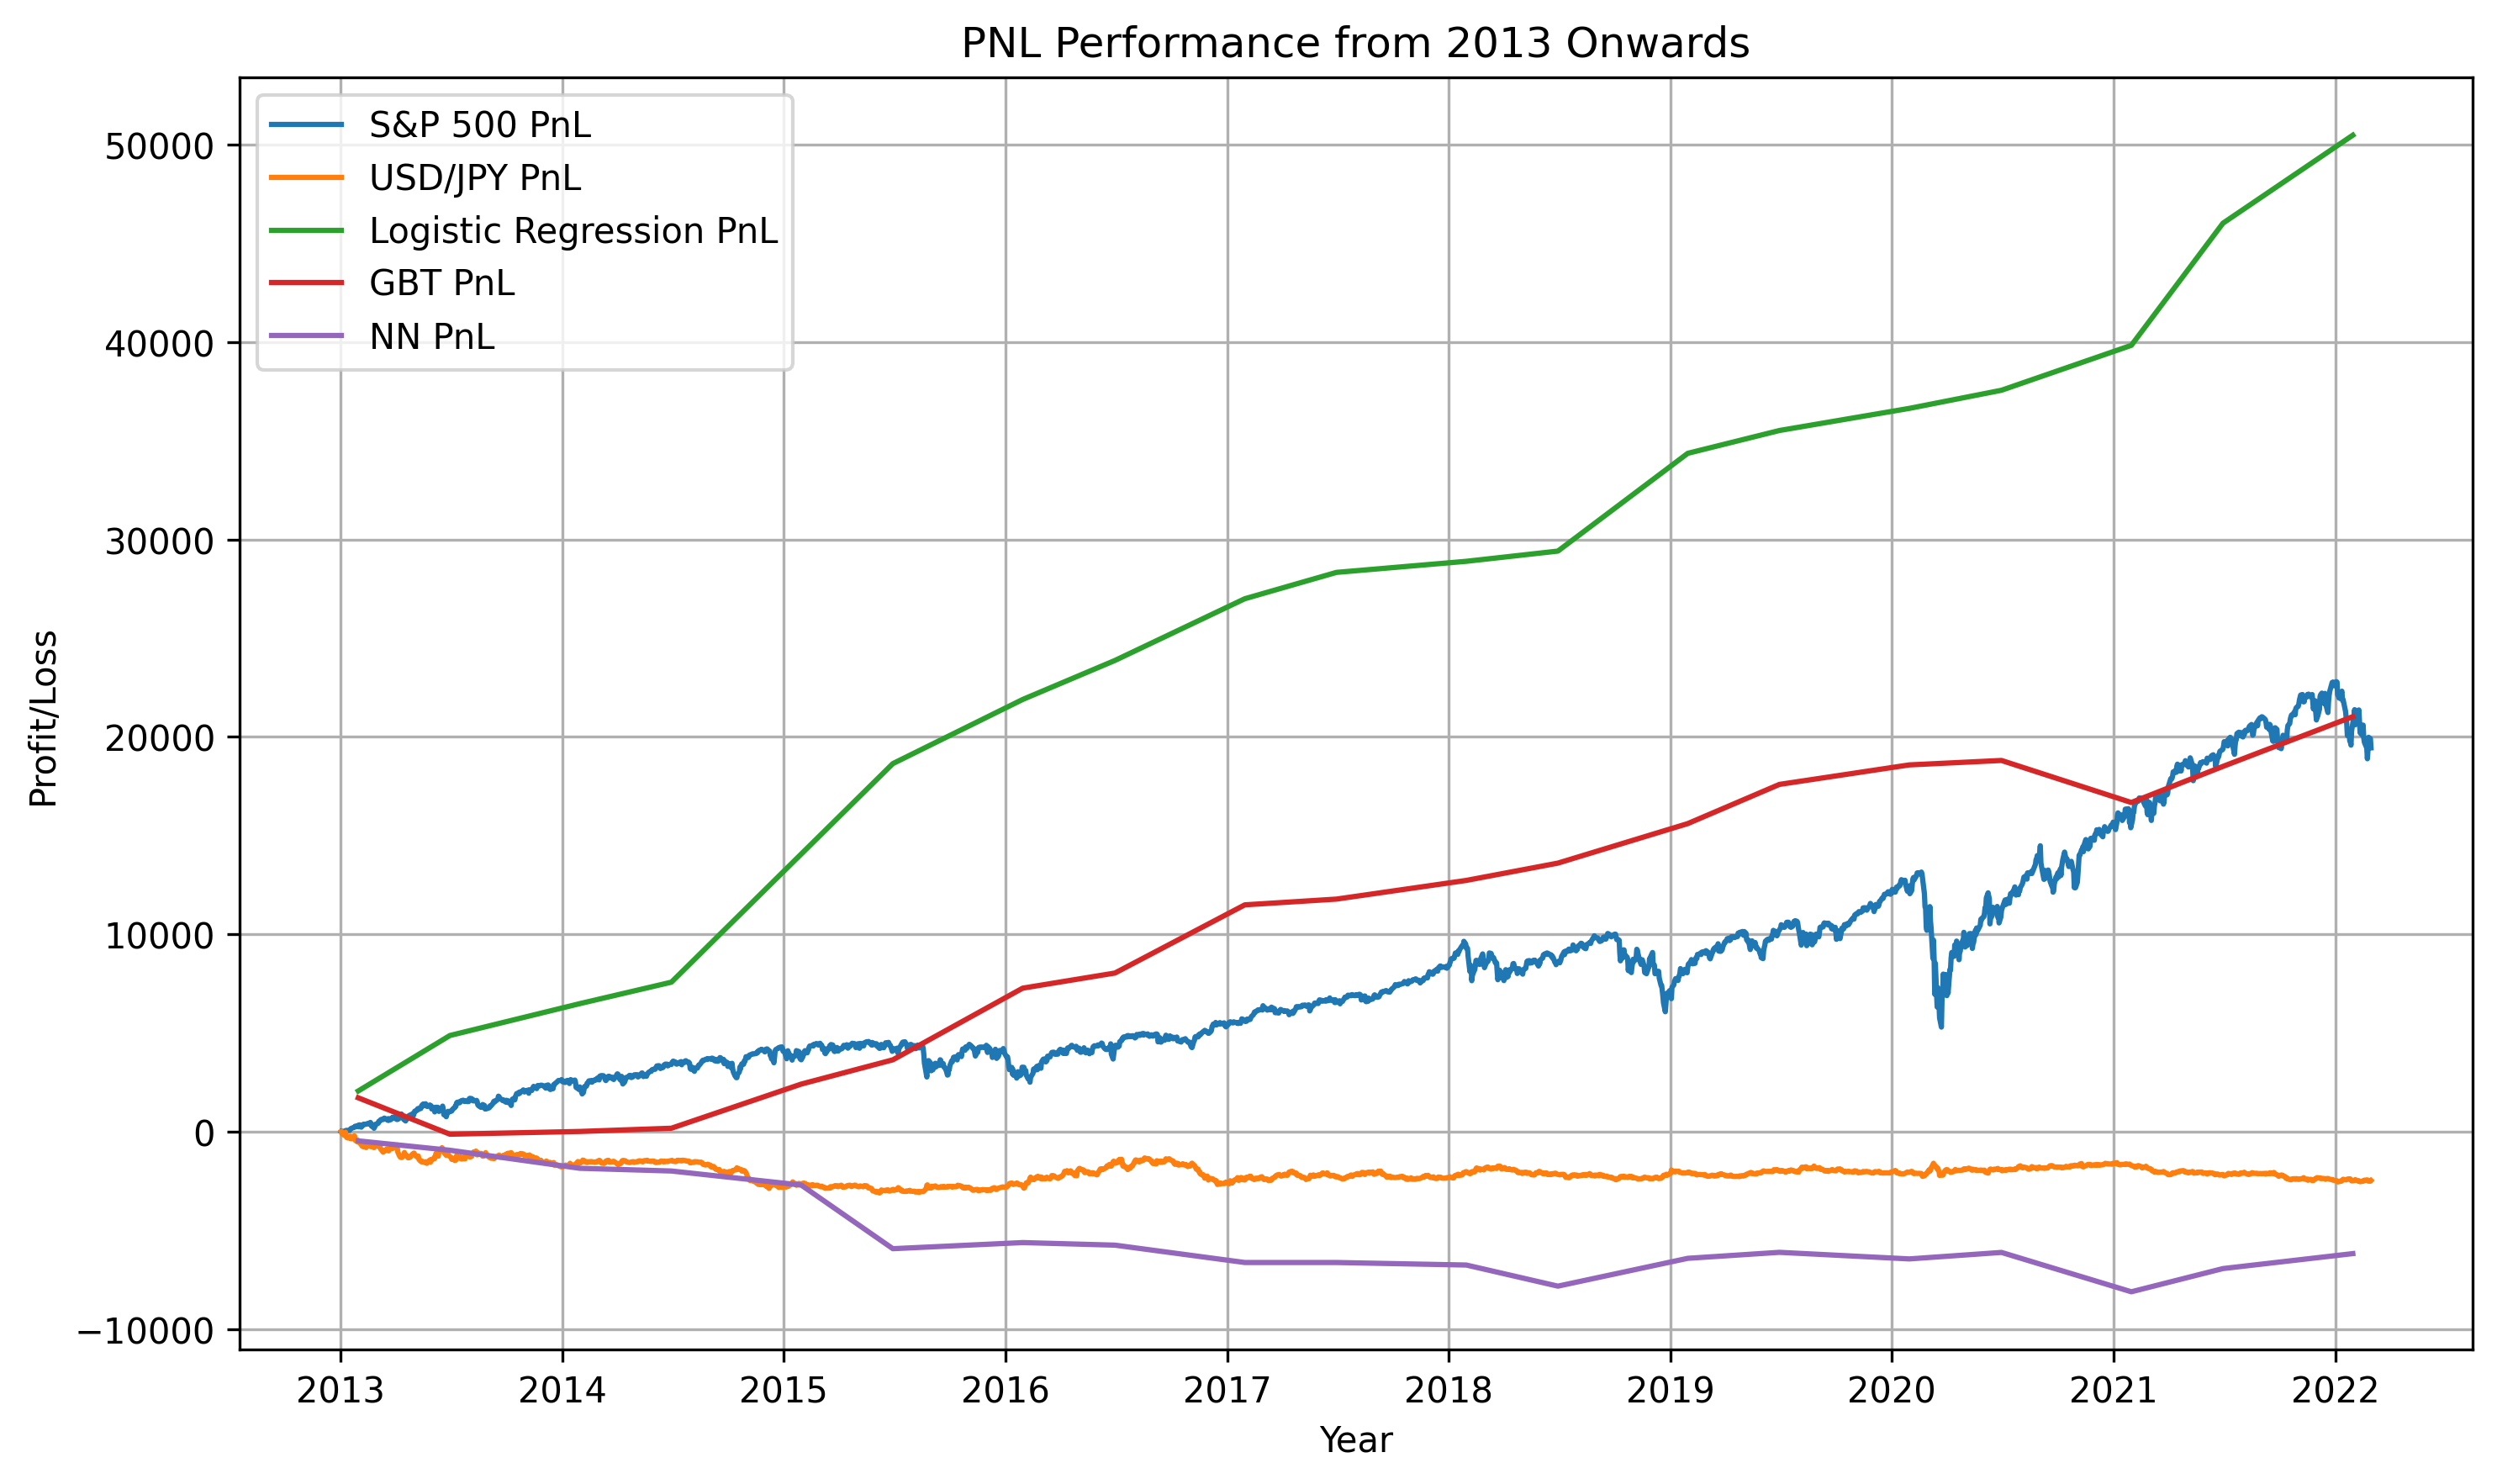
\includegraphics[scale=0.45]{pnl_chartv4.png}
  \caption{PnL Performance Chart Comparing Various Trading Strategies against S\&P500 and Holding JPY Cash}
\end{figure}

\noindent When running all of our models, we generated the PnL distribution shown above. Overall, we can see that Logistic Regression outperformed all other models. It is also worth noting that Gradient Boosted Trees performed similarly to the S\&P500 while Neural Networks gave the worst performance.

\begin{figure}[H]
  \centering
  \includegraphics[scale=0.55]{model_evaluation.png}
  \caption{Evaluation Table of Model Performance Benchmarked Against Forex Movement and S\&P 500}
  \label{fig:chad_salary}
\end{figure}

Notes:
\begin{itemize}
\item Starting portfolio value is 10,000 USD
\item Trading quantum remained fixed at 7,500 USD per lot
\item Returns are displayed in Arithmetic form and not Geometric
\item *For NN the quantum was reset every period due to poor performance
\item PnL evaluated on 4x leverage for consistency
\item PnL Accounts for transaction costs
\item Transaction cost is calculated as 1 USD per trade
\item Aggregate interest costs are computed assuming borrowing rate of 5\% per annum per borrowed quantum
\end{itemize}


\noindent We also conducted testing on different levels of leverage to assess its impact on PnL. We found that in general, there was a linear relationship between leverage and PnL depending on whether the direction was positive or negative. Furthermore we observed possible inflection points in the PnL distribution which could indicate some opportunity for further optimisation when implementing into our models.
\begin{figure}[h]
    \centering
    \includegraphics[scale=0.7]{leverage_vs_pnl_final_2.PNG}
    \caption{Visualisation of PnL against various levels of leverage for each model}
\end{figure}

\newpage
\section{Conclusion}
Non-traditional Technical Indicators may indeed provide some edge in generating buy/sell signal. The ones that rank highly in importance may indicate some movement characteristics of the particular asset class.
\newline
\newline
Out of the signal processing indicators explored, \textbf{Fourier Transform} and \textbf{Kalman Filter} ranked highly, but \textit{not Hurst Exponent}. This could be an affirmation that understanding the cyclical/periodic nature of the USD/JPY trading pair could yield good results. However, understanding the mean-reversion / trend nature of the time series based on recent historical data does not yield added forward predictive signal.
\newline
\newline
Furthermore, traditional Technical Indicators and Econometric Exogenous Variables may prove useful in generating signal when in silo, but may get pushed out when strong, additional indicators are introduced.
\newline
\newline
Though not the crux of our project, we also explored higher derivatives of many of our signal processing and traditional technical indicators. We found that though the indicator's raw values may not rank highly in feature importance, their 1st and/or 2nd derivatives may hold significant importance. In our case, we saw the significance of higher order derivatives of optimised SMA in determining feature importance.
\newline
\newline

\newpage
\section{Appendix}
\subsection{Features List}

\begin{table}[H]
\centering
\begin{tabular}{|p{2cm}|p{4cm}|p{6cm}|}
\hline
\textbf{Category} & \textbf{Indicator} & {Description}\\
\hline
Volatility & Average True Range & EMA of the true range values over a specified period, it indicates the volatility \\
\hline
 {} & Bollinger PercentB & Bollinger band dynamically adjusted to price volatility, and shows signals of overbought and oversold \\
\hline
{} & Bollinger Bandwidth & Difference between upper BB band and lower BB band \\
\hline
{} & BBand Upper & Upper Bollinger band, SMA of N-periods + K times derivatives \\
\hline
{} & BBand Middle & SMA of N-periods \\
\hline
{} & BBand Lower & Lower Bollinger band, SMA of N-periods - K times derivatives \\
\hline
{} & Keltner Channel upper & Keltner Channel upper
KC middle line plus multiple of Average True Range, it identifies the potential trend reversal points \\
\hline
{} & Keltner Channel lower & KC middle line minus multiple of Average True Range, it identifies the potential trend reversal points \\
\hline
{} & Standard Deviation & The standard deviation of asset price, it reflects the volatility \\
\hline
{} & Donchian Channels High & Higher Channel of Donchian Channels, identify the trend and potential reversal \\
\hline
{} & Donchian Channels Low & Lower Channel of Donchian Channels, identify the trend and potential reversal \\
\hline
{} & Chaikin vol & Identify the periods of increased or decreased volatility \\
\hline
Momentum & Awesome Oscillator & Difference between 34-period SMA and 5-period SMA, it identifies the bullish or bearish momentum \\
\hline
{} & Commodity Channel Index & Identify cyclical turns in the price of an asset. It is calculated by dividing Typical Price over Mean Deviation \\
\hline
{} & Momentum & Calculates the difference between today’s closing price and N periods’ ago closing price \\
\hline
\end{tabular}
\end{table}
\begin{table}[h!]
\centering
\begin{tabular}{|p{2cm}|p{4cm}|p{6cm}|}
\hline
\textbf{Category} & \textbf{Indicator} & {Description}\\
\hline
{} & Rate of Change x & percentage change in price between the current closing price and the closing price x periods ago \\
\hline
{} & Rate of Change y & percentage change in price between the current closing price and the closing price y periods ago \\
\hline
{} & Rank Correlation Index (RCI) & Combine price change data and time change data to identify potential changes in market sentiment \\
\hline
Trend & Aroon up & Measure strength of trend by calculating the number of periods since the highest closing price occurred \\
\hline
{} & Aroon down & Measure strength of trend by calculating the number of periods since the lowest closing price occurred \\
\hline
{} & ADX & Reveal the strength of prevailing trend by calculating the division of Average True Range of DX by Smoothing Period \\
\hline
{} & Moving Average & Smooths out the price data and identifies trends of property price \\
\hline
{} & EMA & Smooths out the price data and identifies trends of property price with more weightage allocation to short-term price change \\
\hline
{} & SMA 3 & Moving average using 3 days look back period \\
\hline
{} & EMA 3 & Exponential moving average using 3 days look back period \\
\hline
{} & Weighted MA & Moving average with weighted allocations \\
\hline
{} & Long Moving Avg & Moving average using long look back period \\
\hline
{} & Short Moving Avg 1st Derivative & Gradient of short moving average \\
\hline
{} & Short Moving Avg 2nd Derivative & Curvature of short moving average \\
\hline
{} & Long Moving Avg 1st Derivative & Gradient of long moving average \\
\hline
{} & Long Moving Avg 2nd Derivative & Curvature of long moving average \\
\hline
Oscillator & KDJ K & Difference between Signal line J and K line of Stochastic Oscillator \\
\hline
{} & KDJ D & Difference between Signal line J and D line of Stochastic Oscillator \\
\hline
{} & RSI x & Upper bond of RSI \\
\hline
\end{tabular}
\end{table}
\begin{table}[h!]
\centering
\begin{tabular}{|p{2cm}|p{4cm}|p{6cm}|}
\hline
\textbf{Category} & \textbf{Indicator} & {Description}\\
\hline
{} & RSI y & Lower bond of RSI \\
\hline
{} & RSI & Momentum Oscillator indicator to identify the overbought and oversold signals \\
\hline
{} & Percentage K x & This refers to the K line in the Stochastic Oscillator indicator applied to the x-axis. It measures the current closing price relative to the range of prices over a specific period, signaling potential overbought or oversold conditions in the x-axis market, helping traders identify potential reversal points \\
\hline
{} & Percentage D x & The D line in the Stochastic Oscillator applied to the x-axis, representing a moving average of the K x line. It smoothens the K x line's fluctuations, providing insights into potential trend changes or confirmations of market momentum shifts in the x-axis \\
\hline
{} & Percentage K y & Similar to K x, this indicates the K line in the Stochastic Oscillator applied to the y-axis. It measures the current closing price relative to the range of prices over a specific period, offering insights into potential overbought or oversold conditions in the y-axis market \\
\hline
Other Technical Indicators & Ichimoku Tenkan & Analyse short term market trends and potential reversal point \\
\hline
{} & Ichimoku Kijun & Analyse long term market trends and potential reversal point \\
\hline
{} & MACD & Identify the potential mean reversion \\
\hline
{} & MACD Signal & Signal component of MACD \\
\hline
{} & MACD Line & Line component of MACD \\
\hline
{} & Parabolic SAR & Identify the reversal points in the price direction \\
\hline
{} & Pivot Point & Identify potential support and resistance levels \\
\hline
Non Traditional Technical Indicators & Hurst Exponent & Persistence of current trend using Hurst Exponent \\
\hline
{} & Days Since Peak & Days elapsed since last peak \\
\hline
{} & Days Since Through & Days elapsed since last trough \\
\hline
{} & Price Change Since Peak & Price difference since last peak \\
\hline
{} & Price Change Since Though & Price difference since last through \\
\hline
\end{tabular}
\end{table}
\begin{table}[h!]
\centering
\begin{tabular}{|p{2cm}|p{4cm}|p{6cm}|}
\hline
\textbf{Category} & \textbf{Indicator} & {Description}\\
\hline
{} & Fourier Signal Sell & Sell Signal predicted by Fourier Transformed cycle \\
\hline
{} & Fourier Signal Buy & Buy Signal predicted by Fourier Transformed cycle \\
\hline
{} & Kalman Filter Est & Optimal state estimate of Forex spot rate combining prediction phase and update phase using Kalman Filter Algorithm \\
\hline
{} & Kalman Filter 1st Derivative & The gradient of Kalman Filter \\
\hline
{} & Kalman Filter 2nd Derivative & The curvature of Kalman Filter \\
\hline
Econometric Exogenous Variables & Change of Interest rate Difference & Measure the countries’ Tbill yield \\
\hline
{} & Change of CPI Difference & Measure of a country’s inflation \\
\hline
{} & Change of Current Account Difference & Country’s balance of payments that records its economic transactions with the rest of the world \\
\hline
{} & FDI Difference & Measure of capital inflow to a country \\
\hline
{} & M2 Difference & Measure of money supply in an economy \\
\hline
\end{tabular}
\label{tab:wrapped_text_table}
\caption{All Features Tested During Feature Importance Phase}
\end{table}

\begin{table}[htbp]
    \centering
    \begin{tabular}{p{0.3\textwidth}p{0.6\textwidth}p{0.6\textwidth}} % Adjust the widths as needed
        \hline
        \textbf{Data} & \textbf{Source} \\
        \hline
        Close Prices of USD JPY & Yahoo Finance (Ticker: USDJPY=X)\\
        Close Prices of S\&P500 & Yahoo Finance Package (Ticker: GSPC) \\
        1Y Sovereign Bond Yield & Bloomberg (Tickers: H15T1Y and GJTB12MO)\\
        Consumer Price Index (CPI) & Bloomberg (Tickers: CPI YOY and JNCPIYOY) \\
        Currency Account Balance & Bloomberg (Tickers: OEJPABDO and EHCAUS)\\
        Foreign Direct Investment & Bloomberg (Tickers: FDINUSA and FDINJPN) \\
        Money Supply (M2) & Bloomberg (Tickers: JMNSM2 and ECORUSN) \\
        \hline
    \end{tabular}
    \caption{Data Sources}
\end{table}

\end{document}
